\documentclass[11pt]{article}  
\usepackage[T1]{fontenc}

\usepackage{helvet}
\usepackage{titlesec}
\usepackage[french]{babel}
\usepackage{amsmath,amssymb}
\usepackage{tabu}
\usepackage{url}
\usepackage[svgnames]{xcolor}
\usepackage{graphicx}
\usepackage{geometry}
\usepackage{layout}
\usepackage{listings}
\usepackage{textcomp}
\usepackage{caption}
\usepackage{amsthm}
\usepackage{fancyhdr}
\usepackage{lastpage}
\usepackage{listings}
\usepackage{fontspec}
\usepackage{minted}
\usepackage[toc,page]{appendix} 
\usepackage[nottoc]{tocbibind}
\usepackage{algpseudocode}
\usepackage{algorithm}
\usepackage{algorithmicx}
\usepackage{dirtree}



\newcommand*\DNA{\textsc{dna}}

\newcommand*\Let[2]{\State #1 $\gets$ #2}
\algrenewcommand\algorithmicrequire{\textbf{Precondition:}}
\algrenewcommand\algorithmicensure{\textbf{Postcondition:}}

\floatname{algorithm}{Algorithme}
\renewcommand{\listalgorithmname}{Liste des Algorithmes}



\pagestyle{fancy}
\renewcommand\headrulewidth{1pt}
\fancyhead[L]{Gestion des noeuds isolés en LoRa}
\fancyhead[R]{URCA}
\renewcommand\footrulewidth{1pt}
\fancyfoot[L]{HERARD Joffrey}
\fancyfoot[C]{
\textbf{Page \thepage/\pageref{LastPage}}}
\fancyfoot[R]{2017-2018}
\setlength{\headheight}{14pt}
\renewcommand{\lstlistlistingname}{List of \lstlistingname s}
\renewcommand{\lstlistingname}{Algorithme}
\newenvironment{strechpage}[1][0cm]{%
	\newpage\vspace*{#1}\leavevmode\noindent\centering
	\def\tempdimen{#1}%
	\begin{minipage}{\dimexpr\linewidth-#1-#1\relax}}%
	{\end{minipage}\vspace*\tempdimen\newpage}
	
\renewcommand\appendixpagename{Annexes}	
\renewcommand\appendixname{Annexes}
\renewcommand\appendixtocname{Annexes}




\titleformat{\chapter}[display]
  {\centering\normalfont\huge\bfseries}
  {\chaptertitlename\ \thechapter}
  {20pt}
  {\Huge}
 
\newtheorem{ask}{Question}
\begin{document}

 \makeatletter
\def\maketitle{%
  \null
  \thispagestyle{empty}%
   \vfill
  \begin{center}\leavevmode
    \normalfont
    {\Huge \@title\par}%
    \vskip 3cm
    {\Large \@author\par}%
    \vskip 1cm
    {\Large \@date\par}%
  \end{center}%
  \vfill
  \null
  \cleardoublepage
  }
\makeatother
\title{\begin{center}Projet de fin d'étude:\end{center} Gestion des noeuds isolés en LoRa }
\author{ Joffrey HÉRARD 
\begin{center}Responsable : Olivier FLAUZAC\end{center}}
\date{2017-2018}
\maketitle 
 
\tableofcontents 

\setlength{\parskip}{0.5em}
\newpage
\section{Introduction}
Dans ce rapport, il va être sujet d'aborder les technologies du \textit{LoRaWAN}, du \textit{LoRa} en commencant par definirs ces termes. Ensuite aborder ainsi que expliquer les problémes présent dans une architecture \textit{LoRaWAN} ainsi que les solutions possible pour résoudre ces problèmes. Il va être question avant toute implémentation de faire des simulations sur le modèle de communication \textit{LoRa} avec les algorithme présenter auparavant .Nous allons aborder comment programmer et donc implémenter cette solution dans un capteur. Nous utiliserons notamment dans un premier temps l'implémentation dans des capteurs \textit{LoPy} puis les capteurs \textit{Semtech}. Le rapport ce termineras sur un ensemble de résultats sous forme statistiques et verbales pour commenter ceux-ci.  
\newpage
\section{LoRaWAN}
Comment connecter les milliards de capteurs qui seront potentiellement déployés dans le monde et qui participeront à la construction des villes intelligentes, de la mobilité et de l'industrie du futur ? \newline
Il existe bon nombre de réponses à cette question mais nous pourrons en trouver assurément du côté des LPWAN. Par conséquent nous commenceront par développer ce modèle avant de décrire la spécification de version 1.0 de  \textit{LoRaWAN}, basé sur \textit{LoRa}.
\subsection{Convention de nommage }
Afin de conserver une certaine cohérence vis à vis de la spécification des termes anglo-saxons, nous avons préféré les conserver dans ce document. Toute fois, vous en trouverez une brève définition ci-dessous : 
\begin{itemize}
\item End-devices : Définissent les périphériques cibles comme les capteurs par exemple.
\item Isolated-devices/Isolated Nodes : Définissent les périphériques cibles comme les capteurs par exemple  mais cette fois ci. Isolé par rapport à une gateway  \textit{LoRaWAN}.
\item Uplink : Correspond aux chemins réseaux des end-devices vers le serveur réseaux. 
\item Downlink : Correspond aux chemins réseaux du serveur vers le end-devices. 
\item Gateway : Correspond aux concentrateurs réseaux. 
\item LoRaGateway : Correspond aux concentrateurs réseaux qui sont des end-devices . 
\end{itemize}



\subsection{LPWAN}
Pour certaines applications (villes intelligentes, maintenance prédictive, agriculture connectée, etc.), il s'agit de déployer des centaines de milliers de capteurs (monitoring énergétique, qualité de l'air, gestion des déchets) fonctionnant sur pile et communiquant quotidiennement de très faibles quantités de données, à faible débit vers des serveurs sur Internet (cloud).Les réseaux LPWAN, comme le laisse deviner l'acronyme, sont des réseaux sans fil basse consommation, bas débit et longue portée, optimisés pour les équipements aux ressources limitées pour lesquels une autonomie de plusieurs années est requise. Ces réseaux conviennent particulièrement aux applications qui n'exigent pas un débit élevé.
Contrairement aux opérateurs mobiles les LPWAN utilisent des bandes de fréquences à usage libre, disponibles mondialement et sans licence : ISM (Industriel, Scientifique et Médical). Compte tenu des faibles débits et de la faible occupation spectrale des signaux, il faut en moyenne, pour un réseau LPWAN, 10 fois moins d'antennes pour couvrir la même surface qu'un réseau cellulaire traditionnel.
\subsection{LoRaWAN}
\textit{LoRaWAN} (Long Range Radio Wide Area Network) est un réseau LPWAN basé sur la technologie radio \textit{LoRa}.
Cette technologie, développée par Cycleo en 2009 puis rachetée, 3 ans après, par l'américain Semtech, utilise une technique d'étalement de spectre pour la transmission des signaux radio (chirp spread spectrum). 
La technologie \textit{LoRa}, à travers le réseau  \textit{LoRaWAN}, est poussée par un consortium d'industriels et d'opérateurs nommé \textit{LoRa} Alliance qui regroupe notamment IBM, Cisco, Bouygues Télécom, etc…
\subsubsection{LoRa Alliance}
La \textit{LoRa} Alliance est une association dont le but, non lucratif, est de standardiser le réseau  \textit{LoRaWAN} pour apporter à l'internet des objets (IoT) un moyen fiable pour se connecter à Internet. Cette association a été créée par Semtech et de nombreux acteurs industriels garantissent aujourd'hui l'interopérabilité et la standardisation de la technologie \textit{LoRa}. 







\subsubsection{Les différentes couches d'un réseaux LoRaWAN}
\begin{figure}[h!]
\centering
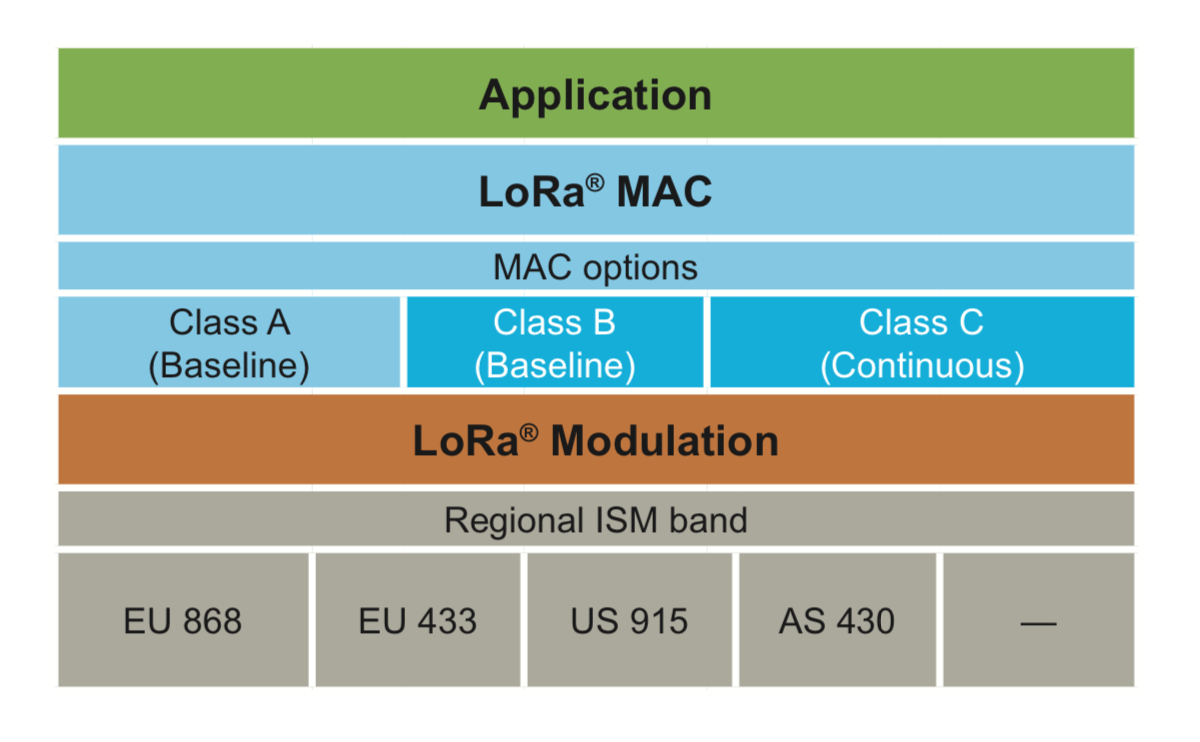
\includegraphics[scale=0.6]{couchelora.png}
\caption{Les différentes couches d'un réseau LoRaWAN}
\end{figure}
On peut alors constater que la couche physique fournie par la technologie \textit{LoRa} n'est pas suffisante pour assurer la communication réseau. En définissant le protocole réseau (\textit{LoRa} MAC), pour une communication d'équipements \textit{LoRa} à travers un réseau, le protocole  \textit{LoRaWAN} assure une communication bi-directionnelle et définit trois classes d'équipements différents. Nous définirons celles-ci dans la partie de notre étude consacrée à l'explication des différences sur les messages, les fenêtres de réception...
\newpage
\subsubsection{Différence entre le LoRa et LoRaWAN}
D'un côté,  \textit{LoRaWAN} est un modèle d'architecture réseaux qui exploite la technologie radio \textit{LoRa} pour faire communiquer les gateways avec les périphériques et les capteurs. En outre, nous détaillerons les particularités de cette architecture réseaux dans le point suivant. A noter, au sein de notre document, la présence de raccourcis d'écriture désignant \textit{LoRa} comme la communication spécifiée en réseau  \textit{LoRaWAN} mais il s'agira bel et bien d'échanges effectués en \textit{LoRa} avec une couche \textit{LoRa} MAC. 
 
\subsubsection{Architecture d'un réseaux LoRaWAN}
\begin{figure}[h!]
\centering
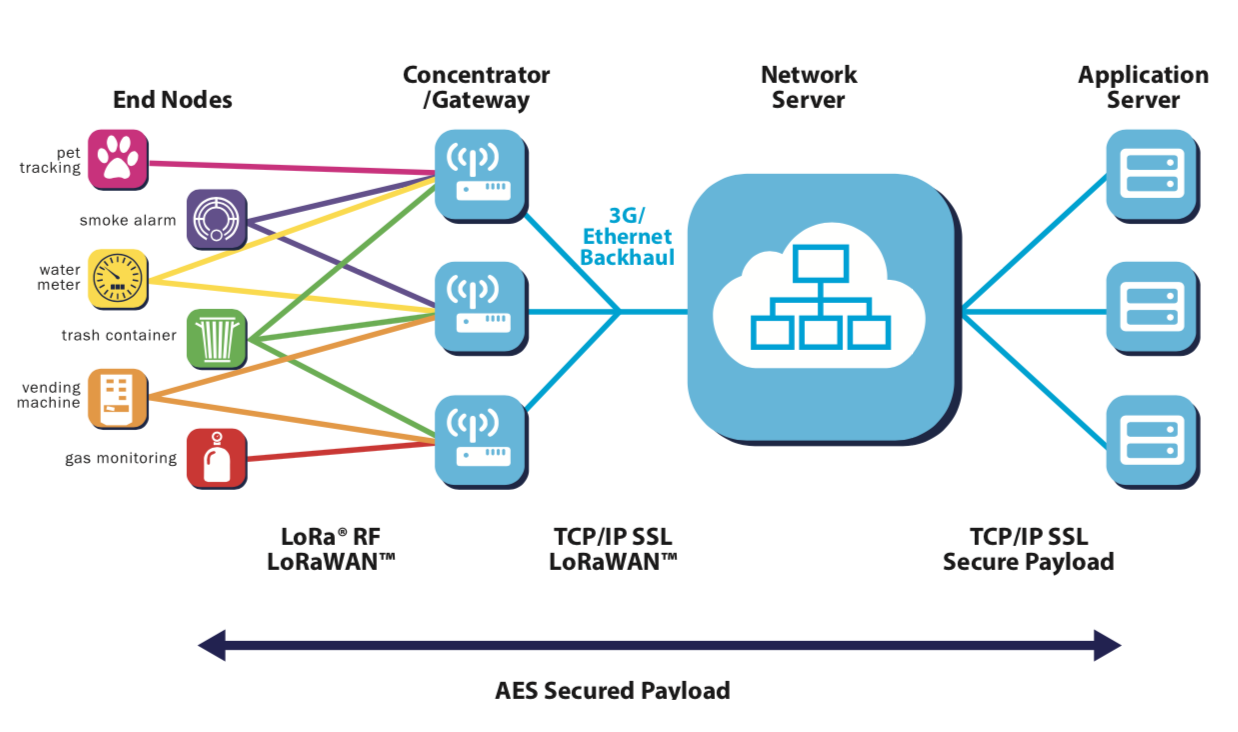
\includegraphics[scale=0.6]{networkArch.png}
\caption{Architecture d'un réseaux LoRaWAN}
\end{figure}
Cette figure représente une architecture classique d'un réseau  \textit{LoRaWAN}. Typiquement un réseau  \textit{LoRaWAN} est en topologie "star of star" étoile en étoile, le centre de cette topologie est le serveur de réseau qui assure la gestion du débit adaptatif, de la sécurité des données ou encore de la redondance des données. Celui ci est entouré d'un côté par les gateways connectés en ethernet/4G au serveur de réseau, auquel les end-devices seront connectés, eux en \textit{LoRa}. D'autre part du serveur réseaux, nous avons les serveur d'applications lié par ethernet, ces mêmes serveur d'application lié elle mêmes à une interface web ( échange HTTP, MQTT).
Une des particularités d’un réseau  \textit{LoRaWAN}, est qu’un équipement ne communique pas exclusivement à travers un concentrateur. Tous les concentrateurs couvrant l’équipement peuvent recevoir les données transmises par ce dernier.
Cela facilite grandement la communication avec les équipements en mobilité en dispensant le réseau de mécanismes de hand-over (passage d’un concentrateur à un autre) qui auraient pour effet de complexifier sa gestion et très probablement de réduire ses performances. Par contre, lorsque le serveur envoie un message à destination d’un équipement, c’est par le biais d’un seul concentrateur. C’est le cas en particulier des messages requérant un acquittement par le serveur.
 assure l'échange entre le serveur de réseaux et les serveurs d'applications : AppsKey. La sécurité après ces serveurs n'est plus géré par la spécification  \textit{LoRaWAN}.
 

\subsubsection{Sécurité d'un réseaux LoRaWAN}
Une question importante est aussi celle de la sécurité a travers le réseaux, on parle de capteurs voir d'un ensemble d'informations qui vont communiqué, donc c'est une question importante, et surtout ça concerne l'Internet des Objets dans son ensemble .
La sécurité est assuré de bout en bout par un chiffrement AES-128 bits, elles sont aux nombre de deux, la première qui couvre les capteurs jusqu'au serveur réseaux nommé NwkSKey.
\begin{itemize}
\item Network Session Key (NwkSKey), assure l’authenticité des équipements sur le réseau .
\item Application Session Key (AppSKey), la sécurité et la confidentialité des données transmises à travers le réseau.
\end{itemize}

En d’autre termes, la clé réseau permet à l’opérateur de sécuriser son réseau alors que la clé applicative permet au fournisseur de l’application de sécuriser les données qui transitent à travers le réseau.

Les données utiles que souhaite transmettre sont tout d’abord chiffrées via la AppSKey. Un en-tête, contenant entre autres l’adresse de l’équipement, est ensuite ajouté aux données chiffrées. À partir de cela, le MIC – Message Integrity Code – est calculé via NwkSKey. Le MIC permet au réseau de vérifier l’intégrité des données et de l’équipement sur le réseau. Enfin, le MIC est ajouté au message contenant l’en-tête et les données chiffrées avant transmission.

À réception du message par le serveur de gestion du réseau, ce dernier pourra vérifier l’intégrité des données grâce au MIC tout en préservant la confidentialité des données (chiffrées par AppSKey).
L'ensemble des trames d'échange vont être décrit dans la suite du document.




\newpage
\subsubsection{Classe A : All end-devices}
\paragraph{Méssage couche physique }
\subparagraph{Messages uplink}
Envoyé par les appareils, reçu par le serveur réseaux et ceux-ci traversant une ou plusieurs stations de base .

\begin{itemize}
\item  Preambule
\item  PHDR : \textit{LoRa} en-tête physique 
\item  PHDR\_CRC : en tête affublé d'une en tête CRC
\item  PHYPayload : Le payload
\item  le champ CRC
\end{itemize}
\subparagraph{Messages downlink}

\begin{itemize}
\item  Preambule
\item  PHDR : \textit{LoRa} en-tête physique 
\item  PHDR\_CRC : en tête affublé d'une en tête CRC
\item  PHYPayload : Le payload
\end{itemize}
\subparagraph{Fenêtre de réception}

Après chaque transmission en uplink, le device ouvre deux fenêtres de réception courtes. Les heures de début de la fenêtre de réception sont des périodes configurées à la fin de la transmission du message au niveau du dernier octet du message .

\subparagraph{Première fenêtre de réception, débit de données, démarrage}

La première fenêtre de réception RX1 utilise le même canal de fréquence que celle du message uplink et un débit de données qui est en fonction du débit de données utilisé pour l'uplink.
RX1 ouvre RECEIVE\_DELAY1 secondes (+/- 20 microsecondes) après la fin de la modulation du message uplink. La relation entre le débit de données de downlink et de l'uplink de RX1 sont spécifique à la région. Par défaut, le premier datarate de la fenêtre de réception est identique à la donnée du dernier message uplink.

\subparagraph{Seconde fenêtre de réception, débit de données, démarrage}
La seconde fenêtre de réception RX2 utilise une fréquence et un débit de données configurables fixes et ouvre RECEIVE\_DELAY2 secondes (+/- 20 microsecondes) après la fin de la modulation d'un message uplink. La fréquence et le débit de données utilisés peuvent être modifiés au moyen des commandes MAC. La fréquence par défaut et le débit de données à utiliser sont spécifiques à la région .

\subparagraph{Durée de la fenêtre}

La durée d'une fenêtre de réception doit être au moins le temps requis par l'émetteur-récepteur radio du device pour détecter efficacement un préambule de message downlink.

\subparagraph{Activité du receveur durant la fenêtre de réception}

Si un préambule est détecté pendant l'une des fenêtres de réception, le récepteur radio reste actif jusqu'à ce que une trame downlink soit démodulée. Si une trame a été détectée et ensuite démodulée pendant la première fenêtre de réception et que la trame était destinée à cet appareil après vérification de l'adresse et du code MIC (message integrity code), le terminal n'ouvre pas la seconde fenêtre de réception.

\subparagraph{Envoi d'un message à travers le réseaux vers un appareil}

Si le serveur réseau à l'intention de transmettre un message uplink , il initiera toujours la transmission précisément au début de l'une de ces deux fenêtres de réception.
\subparagraph{A noté}

Un terminal ne doit pas transmettre un autre message uplink avant qu'il ait reçu un message downlink dans la première ou la deuxième fenêtre de réception de la transmission précédente, ou que la deuxième fenêtre de réception de la transmission précédente ait expiré.

\paragraph{Message couche MAC }
Tout les messages de type uplink et downlink contienne un PHY payload(Payload) cela commence avec un octet d'en tête MAC (MHDR) suivi d'un Payload MAC (MACPayload), et ce termine par 4 octet d'intégrité du code (MIC)

\subparagraph{Couche MAC (PHYPayload)}
La taille maximum M d'un MACPayload est spécifique à la région 


\begin{figure}[h!]
\centering
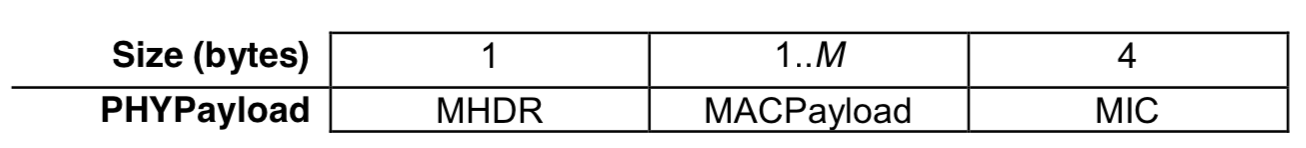
\includegraphics[scale=0.6]{A_phyload.png}
\caption{Format couche MAC}
\end{figure}


\newpage
\subparagraph{En tête MAC. ( MHDR field)}
L'en tête MAC spécifie le type de message (MType) et est encodé par la couche  \textit{LoRaWAN}.
\begin{figure}[h!]
\centering
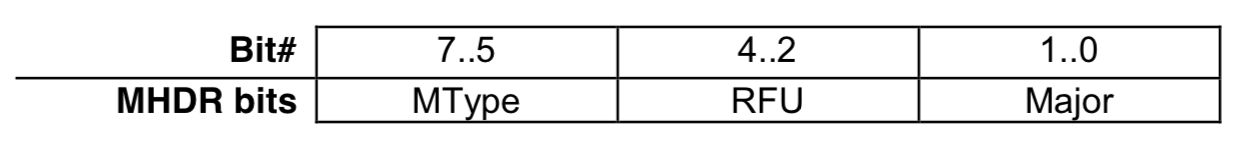
\includegraphics[scale=0.6]{A_mac_header.png}
\caption{En tête MAC}
\end{figure}


\subparagraph{ Type de messages (MType bit field)}
Il y a six messages MAC différents : 
\begin{itemize}
\item join request décrit pour l'utilisation de la procédure "over-the-air activation"
\item join accept décrit pour l'utilisation de la procédure "over-the-air activation"
\item unconfirmed data up/down
\item confirmed data up/down
\end{itemize}

\subparagraph{Données des messages}

Les données des messages sont utilisé pour transféré à la fois les commandes MAC et les données des applications, celles ci peuvent être combiné en un seul message. Un message confirmed-data message doit être accusé de réception par le destinataire cependant un unconfirmed-data message n'en as pas le besoin. Des messages propriétaires peuvent être utilisé pour implémenté des formats de messages non standards qui eux ne sont par inter-opérable avec les messages standards. Ces messages doivent être uniquement utilisé parmi les devices qui ont la même connaissances des ajouts propriétaires.

\subparagraph{ Le payload d'un message sur la couche MAC (MACPayload)}
Le MAC Payload = données du message, sont aussi appellée *data frame*, qui contient une partie d'en tête (FHDR). suivi par un champ optionnel de désignation de port (FPort) mais aussi une partie optionnelle pour un payload (FRMPayload).


\subparagraph{ En-tête (FHDR)}
Le FHDR contient l'adresse de périphérique  (DevAddr), un octet de contrôle de trame (FCtrl), un compteur de trames de 2 octets (FCnt) et jusqu'à 15 octets d'options de trame (FOpts) utilisés pour transporter des commandes MAC .

\subparagraph{Champ du port (Fport)}
Si le champ payload  de la trame n'est pas vide, le champ de port doit être présent. S'il est présent, une valeur FPort de 0 indique que FRMPayload contient uniquement des commandes MAC. Les valeurs FPort 1..223 (0x01..0xDF) sont spécifiques à l'application. Les valeurs FPort 224..255 (0xE0..0xFF) sont réservées aux futures extensions d'application normalisées.

\subparagraph{Chiffrement du Payload sur une trame MAC (FRMPayload)}
Si une trame de données transporte un payload, FRMPayload doit être chiffrée avant l'envoi du  message.
Le code d'intégrité de chiffrement du payload de trame MAC (FRMPayload et MIC) est calculé. Le schéma de chiffrement utilisé est basé sur l'algorithme générique utilisant AES avec une longueur de clé de 128 bits. Par défaut, le chiffrement / déchiffrement est effectué par la couche  \textit{LoRaWAN} pour tous les FPort. Le chiffrement / déchiffrement peut être effectué au-dessus de la couche  \textit{LoRaWAN} pour des FPorts spécifiques sauf 0, si cela est plus pratique pour l'application. Les informations  à partir d'un noeud concernant le protocole de chiffrement / déchiffrement de FPort à l'extérieur de la couche \textit{LoRaWAN} doivent être communiquées au serveur à l'aide d'un canal hors bande .
\subparagraph{calcul du MIC}

msg = MHDR | FHDR | FPort | FRMPayload

le MIC est calculé comme ceci :

cmac = aes128\_cmac(NwkSKey, B0 | msg)
MIC = cmac[0..3]
\paragraph{Commandes MAC}
Pour l'administration de réseau, un ensemble de commandes MAC peut être échangé exclusivement entre le serveur de réseau et la couche MAC d'un périphérique . Les commandes de couche MAC ne sont jamais visibles par l'application, le serveur d'applications ou l'application s'exécutant sur le périphérique .
Une trame de données unique peut contenir n'importe quelle séquence de commandes MAC, greffées dans le champ FOpts ou, lorsqu'elles sont envoyées en tant que trame de données séparée, dans le champ FRMPayload avec le champ FPort défini sur 0. Les commandes MAC superposées sont toujours envoyées sans chiffrement et ne doit pas dépasser 15 octets. Les commandes MAC envoyées en tant que FRMPayload sont toujours chiffrées et ne doivent pas dépasser la longueur FRMPayload maximale.
\paragraph{Activation d'un end-device}
Pour participer dans un réseaux  \textit{LoRaWAN} chaque end-device doit être personalisé et activé.

\subparagraph{Adresse des device (DevAddr)}
32 bits identifient le end-devices dans le réseaux courant.
31-25 = Network ID, 24-0 = NetworkAdress .
les 7 bits de poids forts sont utilisé comme le NwkID .
les 25 derniers sont utiisées pour l'adresse du device qui peut être arbitrairement assigné par l'administrateur réseau .
\subparagraph{Identification de l'application (AppEUI)}
Il identifie le provider de l'application.
\subparagraph{Clé de session réseaux (NwkSkey)}
Elle est spécifique au device utilisé par le serveur réseaux et le device pour calculer l'intégrité de tout les messages.
\subparagraph{Clé de session d'application (AppSKey)}
Elle est spécifique au device utilisé par le serveur réseaux et le device pour chiffré/déchiffré le champ Payload de tout les messages. Mais aussi pour calculer l'intégrité de tout les messages.

\paragraph{Activation avec Over the Air (OTA)}
Les devices doivent forcément utilisé la procédure *join* pour participer aux échanges de données avec le serveur de réseaux. Un device doit forcement utilisé une nouvelle fois le fonction *join* à chaque fois que il a perdu les informations contextuelles lié à la session .
\subparagraph{Identifiant des device (DevEUI)}
l'iddentifiant est au format IEEE EUI64 .
\subparagraph{Clé de l'application(AppKey)}
C'est la clé AES 128 bits.
\subparagraph{Procédure Join}
Consiste en 2 messages MAC entre un device et un serveur de réseau. Ceux-ci sont appelés join request et join accept.
\subparagraph{Message Join-request}
Initialisé par le device en envoyant un message join-request
8 bits AppEUI, 8bits DevEUI, 2bits DevNonce
DevNonce est une valeur aléatoire pour chaque device le serveur de réseaux garde une trace du DevNonce utilisé par les devices dans le passé.  Le serveur de réseaux ignore tout les requêtes de join avec un DevNonce inconnu.
\subparagraph{Méssage Join-accept }
Le serveur renvoie un message join-accept seulement si le device est autorisé à rejoindre le réseaux actuel.
Aucune réponse n'est donné si le device n'est pas autorisé .Le message join-accept contient AppNonce composé  de 3 octets, un identifiant réseau (NetID), une adresse de périphérique (DevAddr), un délai entre TX et RX (RxDelay) et une liste optionnelle de fréquences de canal (CFList ) pour le réseau auquel le device se joint. L'option CFList est spécifique à une région .
\paragraph{Activation par Personallisation }
Le device contient directement le DevAddr, NwkSKey et AppSKey à la place de DevEUI,APPEUI et AppKey.


\newpage
\subsubsection{Classe B : Beacon}
\paragraph{Introduction}
Cette section décrit la couche  \textit{LoRaWAN} Classe B optimisée pour les appareils alimentés par batterie qui peuvent être mobiles ou montés à un emplacement fixe.
Les terminaux doivent mettre en œuvre une opération de classe B lorsqu'il est nécessaire d'ouvrir des fenêtres de réception à des intervalles de temps fixes afin d'activer les messages downlink. L'option \textit{LoRaWAN} Classe B ajoute une fenêtre de réception synchronisée sur le device. L'une des limitations de \textit{LoRaWAN} Class A est la méthode ALOHA d'envoi de données à partir du périphérique; il ne permet pas de connaître le moment de la réaction lorsque l'application client ou le serveur souhaite s'adresser aux périphérique. L'objectif de la classe B est d'avoir un device disponible pour la réception à une heure prévisible, en plus des fenêtres de réception qui suivent la transmission aléatoire d'un méssage uplink du périphérique de classe A. La classe B est obtenue en envoyant à la passerelle un beacon sur une base régulière pour synchroniser tous les devices dans le réseau de sorte que l'appareil puisse ouvrir une courte fenêtre de réception supplémentaire (appelée "ping slot") à un moment prévisible pendant un intervalle de temps périodique.

\paragraph{Principe de la synchronisation du réseaux initialiser en downlink}
Pour qu'un réseau puisse prendre en charge les terminaux de classe B, toutes les passerelles doivent diffuser de manière synchrone un beacon fournissant une référence de synchronisation aux terminaux. Sur la base de cette référence de temporisation, les devices peuvent périodiquement ouvrir des fenêtres de réception, appelées ci-après des intervalles, qui peuvent être utilisées par l'infrastructure de réseau pour initier une communication downlink. Un message downlink utilisant l'un de ces emplacements est appelée un slot-ping. La passerelle choisie pour initier cette communication downlink est sélectionnée par le serveur de réseau sur la base des indicateurs de qualité de signal de la dernière liaison uplink de l'appareil . Pour cette raison, si un périphérique se déplace et détecte une modification de l'identité annoncée dans le beacon reçue, il doit envoyer envoyé en uplink afin que le serveur puisse mettre à jour la base de données du chemin de routage descendant.
Tous les périphériques démarrent et rejoignent le réseau en tant que périphériques de la classe A. L'application peut alors décider de passer à la classe B.


\paragraph{Trame de liaison montante en mode Classe B}
Les trames en uplink en mode Classe B sont identiques aux uplink de classe A à l'exception du bit RFU dans le champ FCtrl de l'en-tête de la trame. Dans l'uplink de classe A, ce bit est inutilisé (RFU). 
\subparagraph{Format de la trame physique}
Un Ping en downlink utilise le même format qu'une trame downlink de classe A, mais pourrait suivre un plan de fréquence de canal différent.
\subparagraph{Messages MAC en Unicast et Multicast}
Les messages peuvent être «unicast» ou «multicast». Les messages monodiffusion sont envoyés à un seul terminal et les messages multidiffusion sont envoyés à plusieurs terminaux. Tous les périphériques d'un groupe de multidiffusion doivent partager la même adresse de multidiffusion et les mêmes clés de chiffrement. La spécification  \textit{LoRaWAN} Classe B ne spécifie aucun moyen pour configurer à distance un tel groupe de multidiffusion ou pour distribuer de manière sécurisée le matériel de clé de multidiffusion requis. Cela doit être effectué pendant la personnalisation du noeud ou via la couche d'application.

\paragraph{Acquisition du beacon et tracking }
Avant de passer de la classe A à la classe B, le device doit d'abord recevoir un beacon pour aligner sa référence d'horloge interne avec le réseau. Une fois en classe B, le périphérique final doit périodiquement rechercher et recevoir un beacon pour annuler toute dérive de son d'horloge interne, par rapport à la synchronisation du réseau. Un périphérique de classe B peut être temporairement incapable de recevoir des beacons (hors de portée des passerelles réseau, présence d'interférences, ..). Dans ce cas, le terminal doit élargir progressivement ses fenêtres de réception de beacon et de ping pour prendre en compte une éventuelle dérive de son horloge interne.
\subparagraph{Temps de fonctionnement minimum sans balise}
En cas de perte de balise, un dispositif est capable de maintenir une opération de classe B pendant 2 heures (120 minutes) après avoir reçu le dernier beacon. Cette opération de classe B temporaire sans beacon est appelée "beacon-less". Il se repose donc sur la propre horloge de l'appareil. Pendant le fonctionnement sans beacon, les slots de réception unicast, multicast et beacon sont tous progressivement étendus pour s'adapter à la possible dérive de l'horloge de l'appareil .
\subparagraph{Extension de l'opération beacon-less à la réception}
Pendant cet intervalle de temps de 120 minutes, la réception de tout beacon dirigée vers l'appareil  prolonge de  120 minutes supplémentaires, car elle permet de corriger toute dérive temporelle et de réinitialiser la durée des créneaux de réception.
\subparagraph{Minimiser la dérive du timing}
Les dispositifs peuvent utiliser la périodicité précise du beacon (lorsqu'elle est disponible) pour calibrer leur horloge interne et réduire ainsi l'imprécision de la fréquence d'horloge initiale. Comme les oscillateurs de synchronisation présentent un décalage de fréquence prévisible, l'utilisation d'un capteur de température pourrait permettre une minimisation supplémentaire de la dérive de la synchronisation.

\paragraph{Synchronisation d'un emplacement en liaison descendante}

\subparagraph{ Définitions}
Pour fonctionner correctement dans la classe B, l'appareil doit ouvrir des créneaux de réception à des instants précis par rapport aux beacon de l'infrastructure.L'intervalle entre le début de deux beacon successif est appelé "beacon period". La transmission de la fenêtre du beacon est alignée avec le début de l'intervalle BEACON\_RESERVED. Chaque beacon est précédée d'un intervalle de temps de garde où aucun emplacement de ping ne peut être placé. Ceci afin d'assurer qu'une downlink initiée pendant une fenêtre de réception juste avant l'heure de garde aura toujours le temps de se terminer sans entrer en collision avec la transmission du beacon. L'intervalle de temps utilisable pour l'intervalle de ping s'étend donc de la fin de l'intervalle de temps réservé aux beacon jusqu'au début de l'intervalle du beacon suivant.
\subparagraph{Emplacement aléatoire}
Pour éviter les collisions systématiques ou les problèmes de congestion, l'index des créneaux horaires est aléatoire et modifié à chaque période de beacon. Les paramètres suivants sont utilisés:
\begin{figure}[h!]
\centering
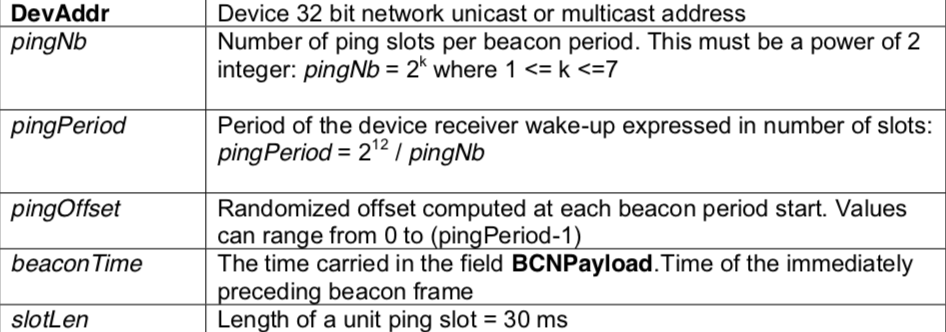
\includegraphics[scale=0.6]{option_random_B.png}
\caption{Options de la classe B}
\end{figure}
A chaque période du beacon, le terminal et le serveur calculent un nouveau décalage pseudo-aléatoire pour aligner les créneaux de réception. Un chiffrement AES avec une clé fixe est utilisé :

Key = 16 x 0x00 

Rand = aes128\_encrypt(Key, beaconTime | DevAddr | pad16)

pingOffset = (Rand[0] + Rand[1]x 256) modulo pingPeriod

\newpage
\begin{figure}[h!]
\centering
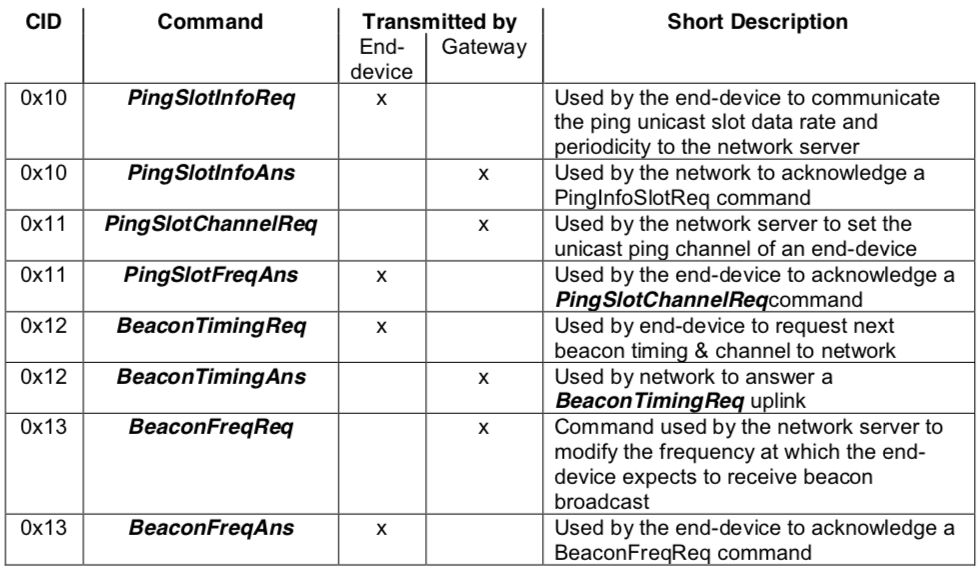
\includegraphics[scale=0.6]{classeB_Mac_Commands.png}
\caption{Commandes de la classe B}
\end{figure}

\paragraph{Beaconing (Option de classe B)}
\subparagraph{ Couche physique de la balise}
En plus de relayer les messages entre les terminaux et les serveurs de réseau, toutes les passerelles participent à la mise en place de mécanismes de synchronisation en envoyant des beacon à des intervalles fixes réguliers configurables par le serveur réseau (BEACON\_INTERVAL). Toutes les balises sont transmises en mode implicite de paquet radio, c'est-à-dire sans entête physique \textit{LoRa} et sans CRC ajouté par la radio. Le préambule de la balise commence par (plus long que par défaut) les symboles non modulés. Cela permet aux dispositifs d'extrémité de mettre en œuvre une recherche par balise à faible puissance. La longueur de la trame du beacon est étroitement liée au fonctionnement de la couche physique radio. Par conséquent, la longueur réelle de la trame peut changer d'une implémentation de région à une autre.

\subparagraph{Format de la trame de Beaconing}

\begin{figure}[h!]
\centering
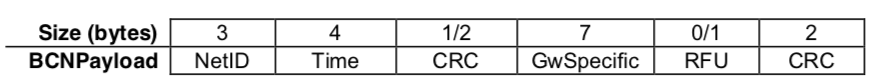
\includegraphics[scale=0.6]{beacon_frame_1.png}
\caption{Trame beacon partie 1}
\end{figure}

\begin{figure}[h!]
\centering
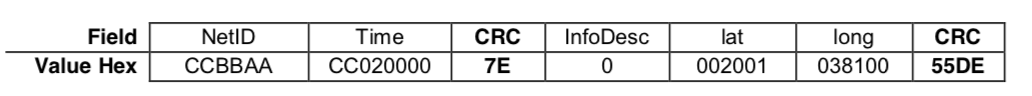
\includegraphics[scale=0.6]{beacon_frame_2.png}
\caption{Trame beacon partie 2}
\end{figure}

\subparagraph{Beaconing : format du champ GwSpecific }

\begin{figure}[h!]
\centering
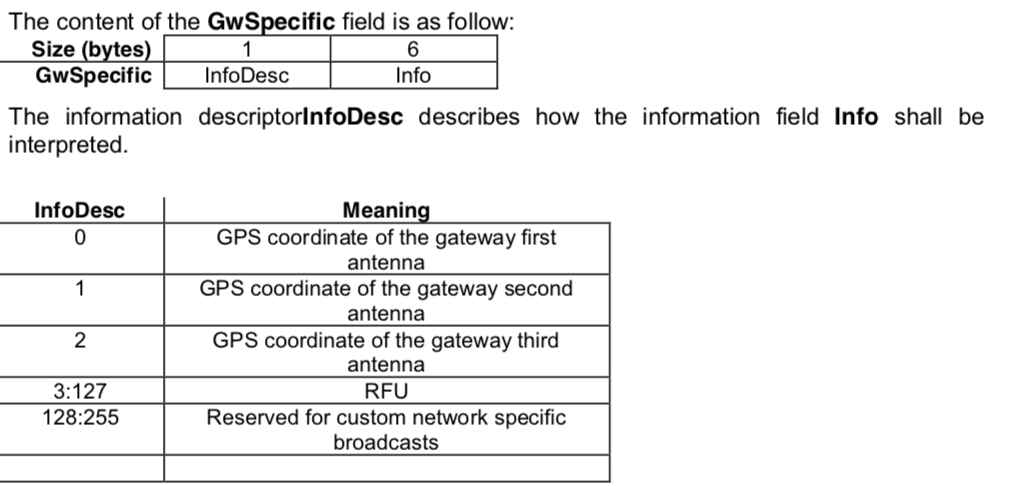
\includegraphics[scale=0.6]{beacon_gwspecific.png} 
\caption{Champ gwspecific}
\end{figure}

\subparagraph{ Gateway coordonées GPS: InfoDesc = 0,1 ou 2}
L'encodage des coordonées GPS sont diffusé dans la balise : 3 octets de lat et 3 octets et Lng, respectivement latitude et longitude
\subparagraph{ Timing précis sur le Beaconing}
Les beacons sont envoyé toute les 128 secondes à partir de minuit UTC 


\newpage
\subsubsection{Classe C : Continiously listening}
Les devices implémentant l'option de classe C sont utilisés pour des applications qui ont une énergie plus que suffisante et n'ont donc pas besoin de minimiser le temps de réception. Les terminaux de classe C ne peuvent pas implémenter l'option de classe B. Le périphérique de classe C écoutera les paramètres des fenêtres RX2 aussi souvent que possible. Le device écoute sur RX2 quand il n'est pas (a) envoyant ou (b) recevant sur RX1, selon la définition de la classe A. Pour ce faire, il ouvrira une petite fenêtre sur les paramètres RX2 entre la fin de la transmission d'un uplink et le début de la fenêtre de réception RX1 et basculera sur les paramètres de réception RX2 dès que la fenêtre de réception RX1 sera fermée; la fenêtre de réception RX2 reste ouverte jusqu'à ce que l'appareil  envoie un autre message.
\subparagraph{Temps de la deuxième fenêtre de réception pour la classe C}
Les périphériques de classe C implémentent les mêmes deux fenêtres de réception que les périphériques de classe A, mais ils ne ferment pas la fenêtre RX2 tant qu'ils n'ont pas besoin d'envoyer à nouveau. Par conséquent, ils peuvent recevoir une liaison descendante dans la fenêtre RX2 à tout moment. Une courte fenêtre d'écoute sur la fréquence RX2 et le débitde donnée est également disponible entre la fin de la transmission et le début de la fenêtre de réception RX1.
\subparagraph{ Multicast liaison descendante}
De même que pour la classe B, les périphériques de classe C peuvent recevoir des trames downlink multicast. L'adresse de multidiffusion et la clé de session de réseau associée et la clé de session d'application doivent provenir de la couche d'application. Les mêmes limitations s'appliquent aux trames downlink multicast de classe C:

* Ils ne sont pas autorisés à transporter des commandes MAC, ni dans le champ FOpt, ni dans le payload sur le port 0, car une liaison descendante multicast n'a pas la même robustesse d'authentification qu'une trame unicast.
* Les bits ACK et ADRACKReq doivent être à zéro. Le champ MType doit porter la valeur de Down Data Unconfirmed Down.
* Le bit FPending indique qu'il y a plus de données de multidiffusion à envoyer. Étant donné qu'un périphérique de classe C conserve son récepteur actif la plupart du temps, le bit FPending ne déclenche aucun comportement spécifique du devices.


\newpage
\section{Problème}
Un problème est relevé après tout ce résumé de la spécification  \textit{LoRaWAN}. Il y a un problème qui se révele assez vite. En effet, le  \textit{LoRaWAN} est basé sur un modèle d'infrastructure. Par exemple, quand est-il d'un noeud qui n'est pas visible par une  \textit{LoRaWAN} Gateway? Il y a deux cas de figures simple : le premier cas est celui  ou le noeud n'est visible d'aucun device et d'aucune gateway  \textit{LoRaWAN}. Dans ce cas il n'y a rien à faire le noeud est isolé de manière permanente. Le deuxième cas de figure est celui qui nous intéresse particulièrement ici, en effet le noeud isolé est visible par un end-device qui lui est à porté d'une  \textit{LoRaWAN} Gateway tout comme l'illustre le schéma suivant :


\begin{figure}[h!]
\centering
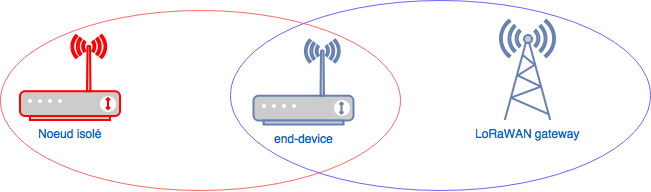
\includegraphics[scale=0.6]{probleme.png} 
\caption{Problème des noeuds isolé}
\end{figure}

\newpage
\section{Solutions}
Il y a  plusieurs piste de solutions afin de résoudre ce problème. Un end node visible par un noeud isolé peut etre redefinie comme une passerelle $\rightarrow$ On définit donc une \textit{LoRa} Gateway (noté LGW à travers le document)
Il y a donc une redéfinition des acteurs :
\begin{itemize}
\item LoRaWAN Gateway (LWGW)
\item LoRa Gateway 
\item Isolated Node (IN)
\end{itemize}

On aurais la possibilité d'avoir deux modes : 
\begin{itemize}
\item Mode proxy : La LoRaGateway fait un relai en aveugle des données des Noeuds Isolés .
\item Mode concentrateur : La LoRaGateway collecte les données des Noeuds Isolés.
\end{itemize}
Il ya tout de même quelque problèmes pour le mode Proxy. 
En effet il y a une certaine compléxité de la mise en oeuvre. Que ce soit au niveau de l'écoute et la captures des échanges par des end-node mais aussi de la capture par le End Node de message du Noeud isolé, ou encore de la capture par le End Node de message à destination du Noeud isolé. Il y a aussi une certaine compléxité au niveau de la gestion des synchronisation en fonction des classes energetique des objets. En classez C, le problème se revele pendant les phases démission du End-Node. En classe A et B lors dez la gestion multiple des slots de réception par le un End Node. Il y a un derniere aspect qui est pratique, en effet les bibliothèques, on écoute et collecte des message sans en etre le destinataire. Il y aurais deux solutions pour pallier à cela, soit la mise en place d'un mode promiscuité, soit d'un recodage complet de la spécification.


Ici nous allons nous intéréssé surtout à l'ensemble des algorithmes soumis par M.Flauzac qui décrive le fonctionnement du mode Concentrateur, afin des les appliquer en  simulation, puis de réaliser la mise en oeuvre/applications de ceux-ci.

\newpage
\subsection{Algorithme}
Cette section va exposé et expliqué l'ensemble des algorithmes présentés.
\subsubsection{Algorithme 1/1 : 1 IN <-> 1 LGW}
\begin{algorithm}
  \caption{ 1/1 : 1 IN <-> 1 LGW}
  \begin{algorithmic}[1]
    \Require{$x$ and $y$ are packed \DNA{} strings of equal length $n$}
    \Statex
    \Function{Distance}{$x, y$}
      \Let{$z$}{$x \oplus y$} \Comment{$\oplus$: bitwise exclusive-or}
      \Let{$\delta$}{$0$}
      \For{$i \gets 1 \textrm{ to } n$}
        \If{$z_i \neq 0$}
          \Let{$\delta$}{$\delta + 1$}
        \EndIf
      \EndFor
      \State \Return{$\delta$}
    \EndFunction
  \end{algorithmic}
\end{algorithm}

\newpage
\subsubsection{Algorithme k/1 : k IN <-> 1 LGW}
\begin{algorithm}
  \caption{ k/1 : k IN <-> 1 LGW}
  \begin{algorithmic}[1]
    \Require{$x$ and $y$ are packed \DNA{} strings of equal length $n$}
    \Statex
    \Function{Distance}{$x, y$}
      \Let{$z$}{$x \oplus y$} \Comment{$\oplus$: bitwise exclusive-or}
      \Let{$\delta$}{$0$}
      \For{$i \gets 1 \textrm{ to } n$}
        \If{$z_i \neq 0$}
          \Let{$\delta$}{$\delta + 1$}
        \EndIf
      \EndFor
      \State \Return{$\delta$}
    \EndFunction
  \end{algorithmic}
\end{algorithm}
\newpage
\subsection{Chronogrammes}
\subsubsection{Phase de découverte et d'enregistrement}
\begin{figure}[h!]
\centering
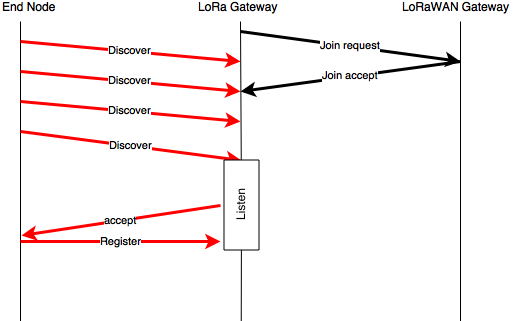
\includegraphics[scale=0.6]{Discovery.png} 
\caption{Phase de découverte}
\end{figure}
\paragraph{Coté Isolated node}Au début le noeud isolé se reveille, il envoie des messages \textbf{Discover}. Si une \textit{LoRa} Gateway répond par un message \textbf{Accept} le noeud répond alors avec un message  \textbf{Register} pour confirmer son appairage avec la \textit{LoRa} Gateway.
\paragraph{Coté LoRa Gateway}
La \textit{LoRa} Gateway avant toute opération avec n'importe quel élement de l'environnement doit s'appairer avec une gateway \textit{LoRaWAN} avec la requete  \textbf{Join Request}.
\paragraph{Coté LoRaWAN Gateway}
La gateway \textit{LoRaWAN} executé un déroulement normal. Elle répond au requete join avec un message  \textbf{Join Accept}
\newpage
\subsubsection{Phase de collecte}
\begin{figure}[h!]
\centering
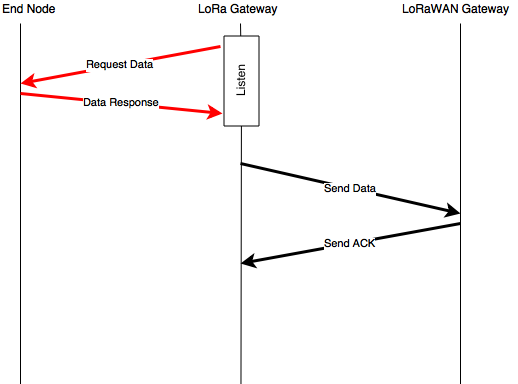
\includegraphics[scale=0.6]{Collect.png} 
\caption{Phase de collecte}
\end{figure}

\paragraph{Coté Isolated node} Le noeud se reveille à un slot prévu entre la \textit{LoRa} Gateway et le noeud. Tout ceci afin de recevoir la demande de donnée de la part de la gateway \textit{LoRa}. Le noeud répond avec les données dans un message nommé  \textbf{Data Response}.
\paragraph{Coté LoRa Gateway}
La \textit{LoRa} Gateway va se reveiller pour collecter les données des noeuds qui lui sont accroché. Elle envoit donc un message  \textbf{Request Data} . Une fois que toutes les données sont reçues, la Gateway assemble les données et envoie à la  \textit{LoRaWAN} gateway. 
\paragraph{Coté LoRaWAN Gateway}
La \textit{LoRaWAN} Gateway accuse la reception des données envoyées par la gateway \textit{LoRa}.
\textbf{Send ACK}


\newpage
\section{Simulation}

\subsection{Le simulateur : Omnet++}
OMNeT ++ est une bibliothèque et une structure de simulation C ++ extensible, modulaire et basée sur des composants, principalement utilisé pour la construction de simulateurs de réseau. Le terme "réseau" est entendu dans un sens plus large qui inclut les réseaux de communication câblés et sans fil, les réseaux sur puce, les réseaux de mise en file d'attente, et ainsi de suite. Les fonctionnalités spécifiques au domaine telles que la prise en charge de réseaux de capteurs, de réseaux ad-hoc sans fil, de protocoles Internet, de modélisation de performances, de réseaux photoniques, etc., sont fournies par des frameworks de modèles, développés en tant que projets indépendants. OMNeT ++ offre un IDE basé sur Eclipse, un environnement d'exécution graphique et une foule d'autres outils. Il existe des extensions pour la simulation en temps réel, l'émulation de réseau, l'intégration de base de données, l'intégration SystemC et plusieurs autres fonctions.
Même si OMNeT ++ n'est pas un simulateur de réseau en soi, il a acquis une grande popularité en tant que plate-forme de simulation de réseau dans la communauté scientifique ainsi que dans les milieux industriels, et a constitué une importante communauté d'utilisateurs.
Afin de réaliser un ensemble de test/simulation nous avons utilisé Omnet pour ce projet.

Le code des fichiers $C^{++}$ est mis à disposition en Annexes.
\subsection{Génération des graphes}
Nous avons choisi d'utiliser iGraph, afin de generer des graphes aléatoire
iGraph est une collection de bibliothèque pour créer et manipuler des graphiques et analyser des réseaux. Il est écrit en C et existe également en tant que paquets Python et R. Il existe de plus une interface pour Mathematica. Le logiciel est largement utilisé dans la recherche universitaire en sciences de réseau et dans des domaines connexes.
igraph a été développé par Gábor Csárdi et Tamás Nepusz. Le code source des paquets iGraph a été écrit en C. iGraph est disponible gratuitement sous GNU General Public License Version 2.

La génération se fait en plusieurs étapes : 
\begin{enumerate}
\item Récupération des arguments : Nombres de  \textit{LoRaWAN} Gateway, \textit{LoRa} Gateway et de Isolated node.	
\item Création du graphe et ajout du nombre de sommets dont on a besoin.
\item On connecte les  \textit{LoRaWAN} à une  \textit{LoRaWAN} gateway, par définitions ils sont enregistré à au moins une gateway  \textit{LoRaWAN}.
\item On connecte des Isolated Node de manière aléatoire à une LoRa Gateway (au moins une)
\item Ensuite on applique un deuxième tour d'association de noeud à des gateway 	basé sur une méthode  Erdös Renyi : On définit la probabilité d'existence entre deux nœuds, pour chaque couple de nœud, on tire au sort un nombre, si le nombre est inférieur on met le lien.
\item On écrit le fichier .ned qui décrit la configuration du graphe crée. 

\begin{minted}[
frame=lines,
framesep=2mm,
baselinestretch=1.2,
bgcolor=LightGray,
fontsize=\footnotesize,
linenos
]{python}
fic.write("\t\t\t" + ""+nomSommet0+"["+str(num_sommet0)+"].channelsO++" + " --> "
+"{delay="+str(delay1)+"ms;}" + " --> " +
""+nomSommet1+"["+str(num_sommet1)+"].channelsI++" + ";\n")
fic.write("\t\t\t" + ""+nomSommet0+"["+str(num_sommet0)+"].channelsI++" + " <-- "
 +"{delay="+str(delay2)+"ms;}" + " <-- " +
   ""+nomSommet1+"["+str(num_sommet1)+"].channelsO++" + ";\n")
\end{minted}

\end{enumerate}
Par exemple voici le résultat graphique réalisé avec GraphViz :

\begin{figure}[!h]
\centering
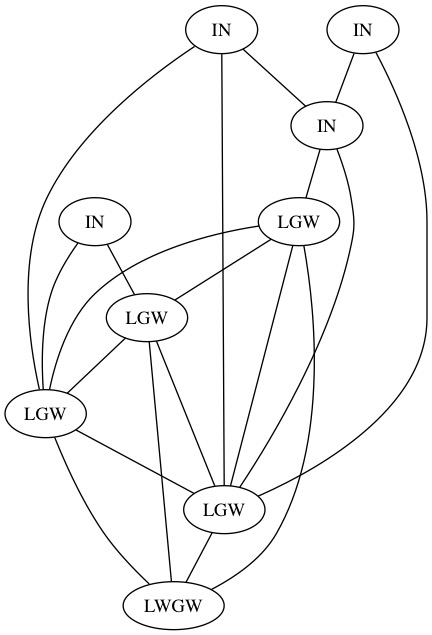
\includegraphics[scale=0.45]{LoRaGraph.jpg} 
\caption{Exemple de Graphe de sortie du script }
\end{figure}
Le code de génération de graphe aléatoire est mis à disposition dans son intégralité en Annexes.
\subsection{Représentation des échanges radio}
Dans cette version purement algorithmique sur Omnet++, la radio est definit par sa porté qui est donc la possibilité de communiqué avec un device. Si une arrête existe alors une communication est possible. Afin d'être plus réaliste, les arrêtes on pour attribut une latence, qui est générer aléatoirement au moment de la création du graphe. La radio étant des ondes quand un device envois un message il l'envoit sur tous les liens qui lui sont attribué.

\begin{figure}[!ht]
\centering
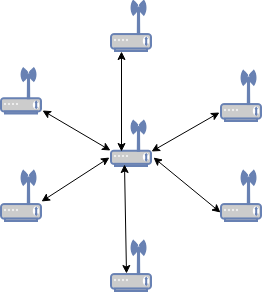
\includegraphics[scale=1]{ex_radio.png} 
\caption{Exemple de communication radio}
\end{figure}


\newpage
\subsection{Exemples de simulations graphiques}
Afin de simplifié, les messages contiennent le nom du message et possedent un code couleur propre et unique. Une \textit{LoRa} Gateway possède une couleur propre à son groupe ( elle même et les Isolated nodes associés), les INs ont aussi cette couleur.
\subsubsection{Simulation sur une chaine}
\begin{figure}[!ht]
\centering
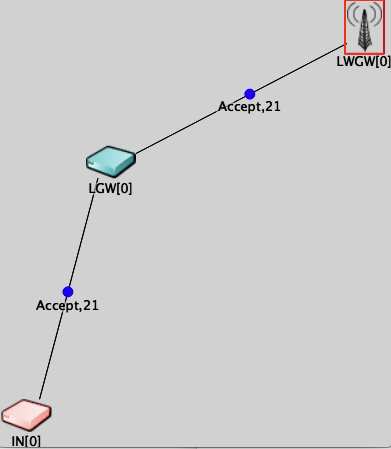
\includegraphics[scale=0.6]{chaine.png} 
\caption{Exemple de chaine}
\end{figure}
Ceci est une image sortie de la simulation graphique, la première réalisé, un exemple typique de chaine avec seulement un élement de chaque composant. C'est le premièr exemple de test réalisé. Ce fut aussi le terrain de devellopement pour affiner le comportement individuel et verifier le fonctionnement correct de chaque composant. Cette simulation ci seras l'exemple typique du première algorithme.
\newpage
\subsubsection{Simulation avec 3 IN sur une LGW}
\begin{figure}[!ht]
\centering
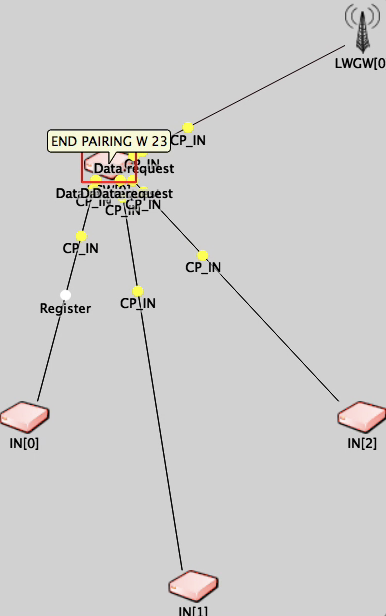
\includegraphics[scale=0.6]{3IN.png} 
\caption{Exemple avec 3 Isolated Nodes}
\end{figure}
Ceci est le deuxième exemple de simulation pour gérer l'enregistrement multiple.Ici nous avons donc toujours une  \textit{LoRaWAN} gateway qui est connecté a une \textit{LoRa} Gateway qui doit gérer trois Isolated Node Cette simulation ci seras l'exemple typique du deuxième algorithme.
\newpage
\subsubsection{Simulation à plus grande echelle }
\begin{figure}[!ht]
\centering
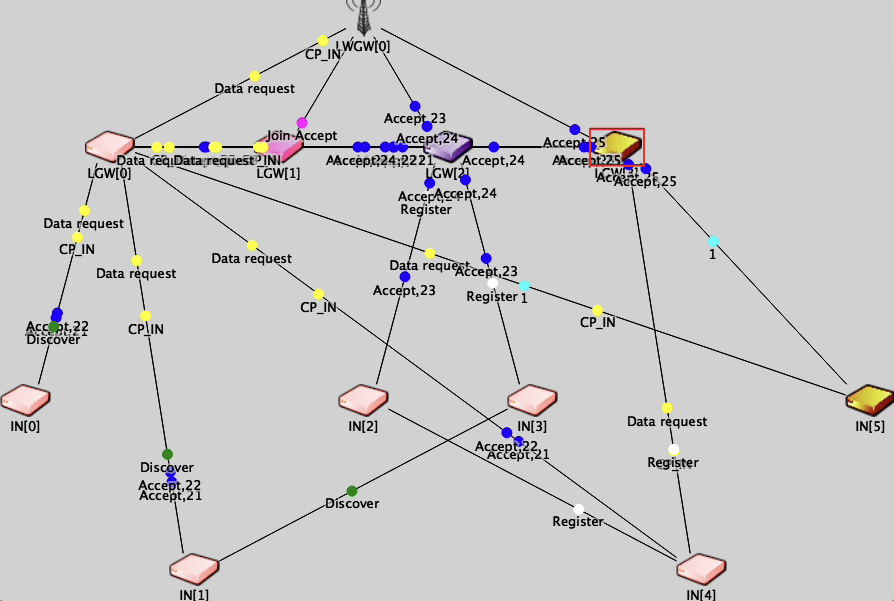
\includegraphics[scale=0.45]{fat.png} 
\caption{Exemple à grande echelle}
\end{figure}
Ceci est le troisème exemple de simulation pour gérer l'enregistrement multiple ainsi que l'unicité d'un enregistrement sur une Gateway \textit{LoRa} d'un device.Ici nous avons donc toujours une  \textit{LoRaWAN} gateway qui est connecté a quatre \textit{LoRa} Gateway qui doit gérer X Isolated Node Cette simulation ci seras l'exemple typique du deuxième algorithme. Mais aussi d'un troisème cas de figure possible. Cette exemple est surtout présent pour montrer et pousser la simulation à être plus proche de la réalité.
L'exemple présenté ci-contre fait aussi transparaitre les exemples ou les communications sont difficiles. Un noeud peut pendant un certain temps ne faire que envoyer des messages \textbf{Discover} très longtemps. Pour plusieurs raisons, notamment celle-ci : 
\begin{itemize}
\item Problème de latence sur le reseaux de communication. 
\item Problème de bruit radio (Plusieurs emissions sont réalisé en même temps de la part de plusieurs device, que ce soit sur le device de recepetion ou d'émission provocant la corrupition des messages)
\item Problème de phase réception, en effet des slots sont prévue ainsi que deux fenêtre de réception dans la specification \textit{LoRa}. Il se peut que deux device pas encore synchroniser est du mal à l'être .
\end{itemize}
\newpage
\section{Programmation}

\subsection{LoPy}
\subsection{Semtech}
\newpage
\section{Résultats}
\newpage
\section{Conclusion}
TO DO 
\newpage
\listoffigures
\newpage
\listofalgorithms
\addcontentsline{toc}{section}{Liste des algorithmes}
\newpage
\begin{appendices} 
\section{Code iGraph} 
\inputminted{python}{../igraph/loraGraph.py}
\newpage
\section{Code Omnet++} 
\subsection{Fichier .h}
\inputminted[
frame=lines,
framesep=2mm,
baselinestretch=1.2,
bgcolor=LightGray,
fontsize=\footnotesize,
linenos
]{c++}{../src/frequency.h}

\newpage

\inputminted[
frame=lines,
framesep=2mm,
baselinestretch=1.2,
bgcolor=LightGray,
fontsize=\footnotesize,
linenos
]{c++}{../src/IsoN.h}


\newpage

\inputminted[
frame=lines,
framesep=2mm,
baselinestretch=1.2,
bgcolor=LightGray,
fontsize=\footnotesize,
linenos
]{c++}{../src/LGW.h}


\newpage

\inputminted[
frame=lines,
framesep=2mm,
baselinestretch=1.2,
bgcolor=LightGray,
fontsize=\footnotesize,
linenos
]{c++}{../src/LWGW.h}


\newpage

\inputminted[
frame=lines,
framesep=2mm,
baselinestretch=1.2,
bgcolor=LightGray,
fontsize=\footnotesize,
linenos
]{c++}{../src/messageLoRA.h}
\newpage
\subsection{Fichier .cpp}
L'intégralité des codes se trouve dans l'archive jointe au présent rapport : 
\newpage
\section{Arborescence des fichiers} 
\dirtree{%
 .1 Racine du projet.
  .2 omnetpp.ini .
  .2 Makefile .
  .2 README.md .
  .2 igraph .
   .3 loraGraph.py .
   .3 README .
  .2 out .
   .3 clang-debug .
    .4 src .
     .5 Fichier de debug.
   .3 clang-release .
    .4 src .
     .5 Fichier de release.
  .2 old .
   .3 src .
    .4 Ancien fichier source d'une ancienne méthode d'enregistrement des noeuds.
  .2 results .
  .2 lopy .
   .3 README.md .
   .3 test .
    .4 Fichiers de tests .
   .3 current .
    .4 IsolatedNode.py .
    .4 messageLoRa.py .
    .4 LoRaGateway.py .
    .4 nota\_DO\_NOT\_DELETE.txt .
  .2 simulations .
   .3 omnetpp.ini .
   .3 network.ned .
   .3 lora.ned .
   .3 run .
   .3 package.ned .
  .2 Rapport\_PFE .
   .3 Rapport.pdf.
  .2 src .
   .3 Code source de Omnet++.
}


\end{appendices} 

\end{document}